\begin{apendicesenv}

  % % Imprime uma página indicando o início dos apêndices
  \partapendices
  % % Para cada apêndice, um \chapter


  \chapter{Translated Survey Questionnaire}\label{appendix:questionnaire}

  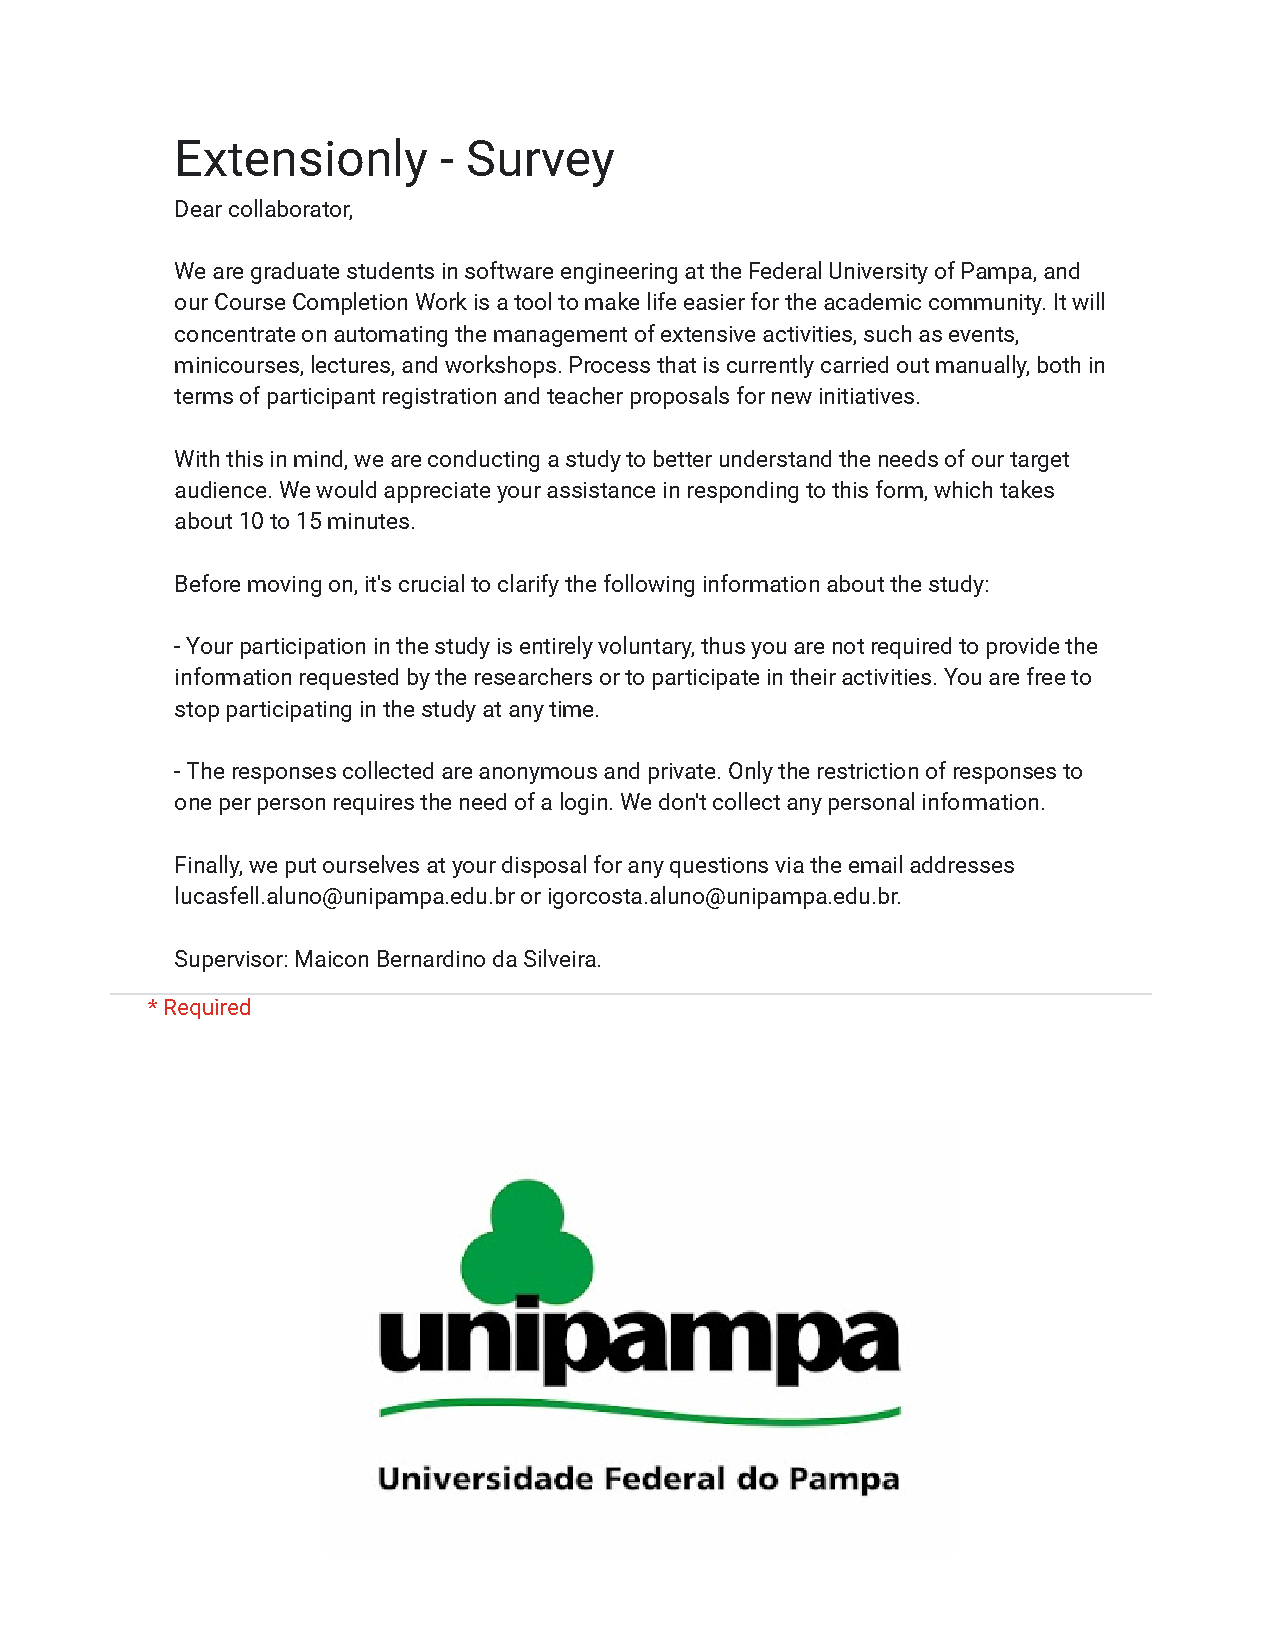
\includepdf[pages={1-23}]{artifacts/5-questionnaire-en.pdf}

  % De acordo com a ABNT:

  % \begin{quotation}
  % Apêndice (opcional): texto utilizado quando o autor pretende complementar sua argumentação. São identificados por letras maiúsculas e travessão, seguido do título. Ex.: APÊNDICE A - Avaliação de células totais aos quatro dias de evolução

  % Anexo (opcional): texto ou documento \textbf{não elaborado pelo autor} para comprovar ou ilustrar. São identificados por letras maiúsculas e travessão, seguido do título. Ex.: ANEXO A - Representação gráfica de contagem de células
  % \end{quotation}

  % Tais definições (e outras) podem ser encontradas na NBR 14724-2001 Informação e documentação - trabalhos acadêmicos\footnote{http://www.firb.br/abntmonograf.htm}.


  % %==============================================================================
  % \chapter{Segundo Apêndice}
  % %==============================================================================

  % Pode ser que tenha outro...


\end{apendicesenv}
